\documentclass[tikz]{standalone}
\usetikzlibrary{arrows.meta, positioning}

\begin{document}
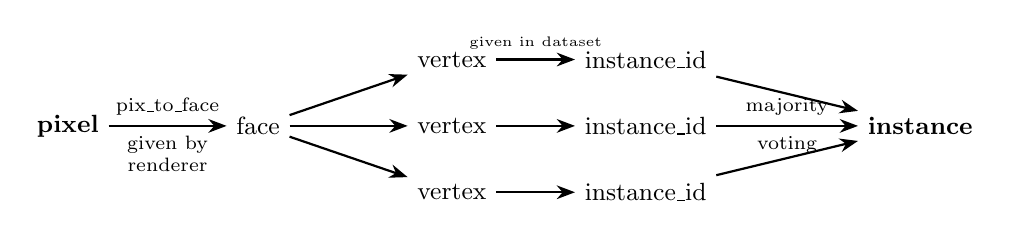
\begin{tikzpicture}[
    node distance=1.2cm and 1.5cm,
    every node/.style={font=\small},
    arrow/.style={-{Stealth}, thick}
]
    % (Paste the TikZ code here from the previous response)
    \node (pixel) {\textbf{pixel}};
    \node (face) [right=of pixel] {face};
    \node (v2) [right=of face] {vertex};
    \node (v1) [above=0.4cm of v2] {vertex};
    \node (v3) [below=0.4cm of v2] {vertex};
    \node (id1) [right=1cm of v1] {instance\_id};
    \node (id2) [right=1cm of v2] {instance\_id};
    \node (id3) [right=1cm of v3] {instance\_id};
    \node (inst) [right=1.8cm of id2] {\textbf{instance}};

    \draw [arrow] (pixel) -- node[above, font=\scriptsize] {pix\_to\_face} 
                             node[below, font=\scriptsize, align=center] {given by\\ renderer} (face);
    \draw [arrow] (face) -- (v1);
    \draw [arrow] (face) -- (v2);
    \draw [arrow] (face) -- (v3);
    \draw [arrow] (v1) -- node[above, pos=0.5, font=\tiny, sloped] {given in dataset} (id1);
    \draw [arrow] (v2) -- (id2);
    \draw [arrow] (v3) -- (id3);
    \draw [arrow] (id1) -- (inst);
    \draw [arrow] (id2) -- node[above, font=\scriptsize, align=center] {majority}
                           node[below, font=\scriptsize, align=center] {voting} (inst);
    \draw [arrow] (id3) -- (inst);
\end{tikzpicture}
\end{document}